\subsection{Use Case}
    \subsubsection{Danh sách Use Case}
        \begin{figure}[H]
	\centering
	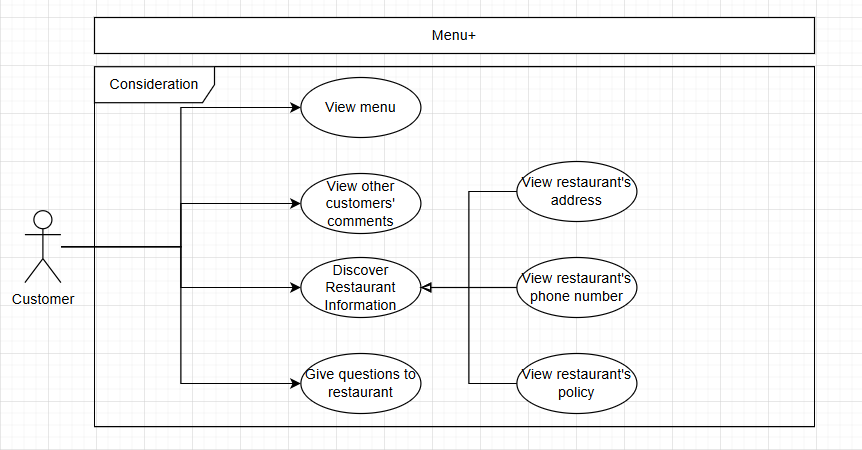
\includegraphics[width=\linewidth]{Images/ucd-consideration.png}
	\caption{Usecase Diagram giai đoạn Consideration}
        \end{figure}
        
        \begin{longtable}{|p{1cm}|p{5cm}|p{9cm}|}
        \hline
        \textbf{\#} & \textbf{Tên Use Case} & \textbf{Mô tả} \\ 
        \hline
        \endfirsthead
        \hline
        \textbf{\#} & \textbf{Tên Use Case} & \textbf{Mô tả} \\ 
        \endhead
        \hline
        % \multicolumn{3}{|r|}{\small\slshape Còn tiếp} \\ \hline
        \endfoot
        \hline
        \endlastfoot
        1 & Xem thực đơn & Khách hàng có thể xem danh sách các món ăn có sẵn trong thực đơn của nhà hàng, bao gồm thông tin về món ăn như giá cả, mô tả và hình ảnh. \\ 
        \hline
        2 & Xem bình luận của khách hàng khác & Khách hàng có thể xem các đánh giá, nhận xét từ những khách hàng trước đó về món ăn, dịch vụ hoặc trải nghiệm tại nhà hàng. \\ 
        \hline
        3 & Khám phá thông tin nhà hàng & Khách hàng có thể tìm hiểu các thông tin cơ bản về nhà hàng như lịch sử, phong cách ẩm thực, giờ mở cửa, và các thông tin liên quan khác. Có thể xem địa chỉ, số điện thoại, chính sách nhà hàng.\\ 
        \hline
        4 & Đặt câu hỏi cho nhà hàng & Khách hàng có thể gửi câu hỏi trực tiếp đến nhà hàng để hỏi về thực đơn, dịch vụ, hoặc các thông tin khác mà họ quan tâm. \\ 
        \hline
        \caption{Danh sách Use Case trong giai đoạn Consideration}\\
        \end{longtable}

        \begin{figure}[H]
	\centering
	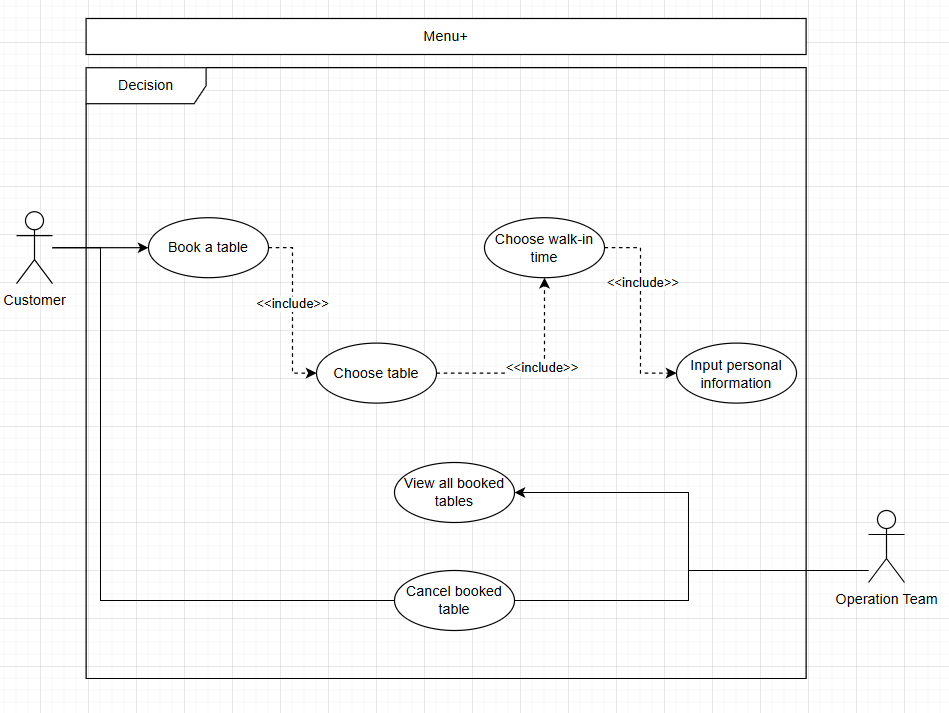
\includegraphics[width=\linewidth]{Images/ucd-decision.png}
	\caption{Usecase Diagram giai đoạn Decision}
        \end{figure}
        
        \begin{longtable}{|p{1cm}|p{5cm}|p{9cm}|}
        \hline
        \textbf{\#} & \textbf{Tên Use Case} & \textbf{Mô tả} \\ 
        \hline
        \endfirsthead
        \hline
        \textbf{\#} & \textbf{Tên Use Case} & \textbf{Mô tả} \\ 
        \endhead
        \hline
        % \multicolumn{3}{|r|}{\small\slshape Còn tiếp} \\ \hline
        \endfoot
        \hline
        \endlastfoot
        5 & Đặt bàn & Khách hàng có thể đặt bàn trước khi đến nhà hàng, bao gồm việc chọn thời gian và số lượng người trong nhóm. Khi đặt bàn, Khách hàng có thể chọn được bàn, thời gian đến và thông tin cá nhân. \\ 
        \hline
        6 & Xem danh sách bàn đã đặt & Nhân viên vận hành (Operation Team) có thể xem danh sách các bàn đã được đặt bởi khách hàng, bao gồm thời gian và thông tin khách hàng. \\ 
        \hline
        7 & Hủy đặt bàn & Khách hàng hoặc nhân viên vận hành có thể hủy một đặt bàn đã được thực hiện trước đó nếu khách hàng không còn nhu cầu. \\ 
        \hline
        \caption{Danh sách Use Case trong giai đoạn Decision}\\
        \end{longtable}

        \begin{figure}[H]
	\centering
	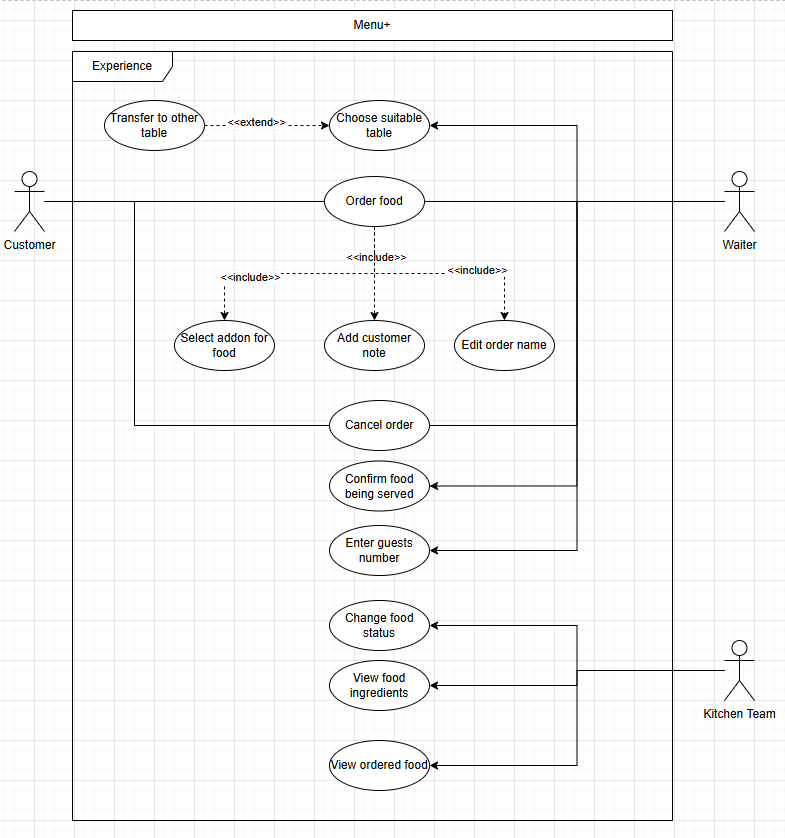
\includegraphics[width=\linewidth]{Images/ucd-experience.png}
	\caption{Usecase Diagram giai đoạn Experience}
        \end{figure}

        \begin{longtable}{|p{1cm}|p{5cm}|p{9cm}|}
        \hline
        \textbf{\#} & \textbf{Tên Use Case} & \textbf{Mô tả} \\ 
        \hline
        \endfirsthead
        \hline
        \textbf{\#} & \textbf{Tên Use Case} & \textbf{Mô tả} \\ 
        \endhead
        \hline
        % \multicolumn{3}{|r|}{\small\slshape Còn tiếp} \\ \hline
        \endfoot
        \hline
        \endlastfoot
        8 & Chuyển đến bàn khác & Nhân viên phục vụ có thể chuyển khách sang một bàn khác nếu bàn hiện tại không phù hợp hoặc có yêu cầu đặc biệt. \\ 
        \hline
        9 & Đặt món ăn & Khách hàng hoặc nhân viên phục vụ có thể đặt món ăn từ thực đơn, bao gồm các bước như chọn món, thêm ghi chú tùy chỉnh và xác nhận đơn hàng. \\ 
        \hline
        10 & Sửa tên đơn hàng & Nhân viên phục vụ (Waiter) có thể sửa tên đơn hàng để dễ dàng nhận diện, ví dụ: gắn tên khách hàng hoặc số bàn vào đơn hàng. \\ 
        \hline
        11 & Hủy đơn hàng & Khách hàng hoặc nhân viên phục vụ có thể hủy đơn hàng nếu khách hàng không còn muốn đặt món đó nữa. \\ 
        \hline
        12 & Xác nhận món ăn được phục vụ & Nhân viên phục vụ xác nhận rằng món ăn đã được phục vụ đến khách hàng, đảm bảo đơn hàng hoàn tất. \\ 
        \hline
        13 & Nhập số lượng khách & Khách hàng hoặc nhân viên phục vụ nhập số lượng khách trong nhóm để đảm bảo nhà hàng chuẩn bị đủ chỗ ngồi và phục vụ phù hợp. \\ 
        \hline
        14 & Thay đổi trạng thái món ăn & Đội bếp (Kitchen Team) có thể cập nhật trạng thái món ăn, ví dụ: đang chuẩn bị, đã hoàn thành, đã phục vụ, v.v. \\ 
        \hline
        15 & Xem nguyên liệu món ăn & Đội bếp có thể xem danh sách nguyên liệu của món ăn để chế biến đúng thành phần, công thức món ăn. \\ 
        \hline
        16 & Xem món ăn đã đặt & Đội bếp có thể xem danh sách các món ăn đã đặt, bao gồm trạng thái của từng món được sắp xếp theo thứ tự ưu tiên để kịp thời hoàn thành món. \\ 
        \hline
        \caption{Danh sách Use Case trong giai đoạn Experience}\\
        \end{longtable}

        \begin{figure}[H]
	\centering
	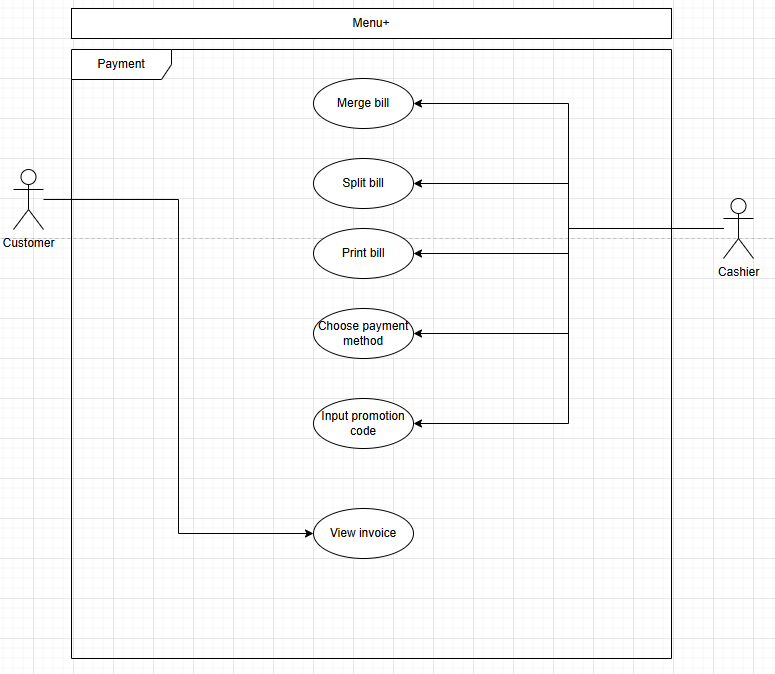
\includegraphics[width=\linewidth]{Images/ucd-payment.png}
	\caption{Usecase Diagram giai đoạn Payment}
        \end{figure}

        \begin{longtable}{|p{1cm}|p{5cm}|p{9cm}|}
        \hline
        \textbf{\#} & \textbf{Tên Use Case} & \textbf{Mô tả} \\ 
        \hline
        \endfirsthead
        \hline
        \textbf{\#} & \textbf{Tên Use Case} & \textbf{Mô tả} \\ 
        \endhead
        \hline
        % \multicolumn{3}{|r|}{\small\slshape Còn tiếp} \\ \hline
        \endfoot
        \hline
        \endlastfoot
        17 & Gộp hóa đơn & Nhân viên thu ngân (Cashier) có thể gộp nhiều hóa đơn thành một hóa đơn duy nhất để thanh toán. \\ 
        \hline
        18 & Tách hóa đơn & Nhân viên thu ngân có thể tách hóa đơn thành nhiều phần để thanh toán riêng lẻ, ví dụ: chia đều cho từng người trong nhóm. \\ 
        \hline
        19 & In hóa đơn & Nhân viên thu ngân có thể in hóa đơn cho khách hàng sau khi thanh toán, bao gồm chi tiết các món ăn và tổng số tiền. \\ 
        \hline
        20 & Chọn phương thức thanh toán & Nhân viên thu ngân có thể chọn phương thức thanh toán (tiền mặt, thẻ tín dụng, ví điện tử, v.v.) để thanh toán hóa đơn. \\ 
        \hline
        21 & Nhập mã khuyến mãi & Nhân viên thu ngân có thể nhập mã khuyến mãi ưu đãi hoặc giảm giá trên hóa đơn thanh toán. \\ 
        \hline
        22 & Xem hóa đơn & Khách hàng hoặc nhân viên thu ngân có thể xem chi tiết hóa đơn, bao gồm danh sách món ăn, giá tiền, và các khoản giảm giá (nếu có). \\ 
        \hline
        \caption{Danh sách Use Case trong giai đoạn Payment}\\
        \end{longtable}

        \begin{figure}[H]
	\centering
	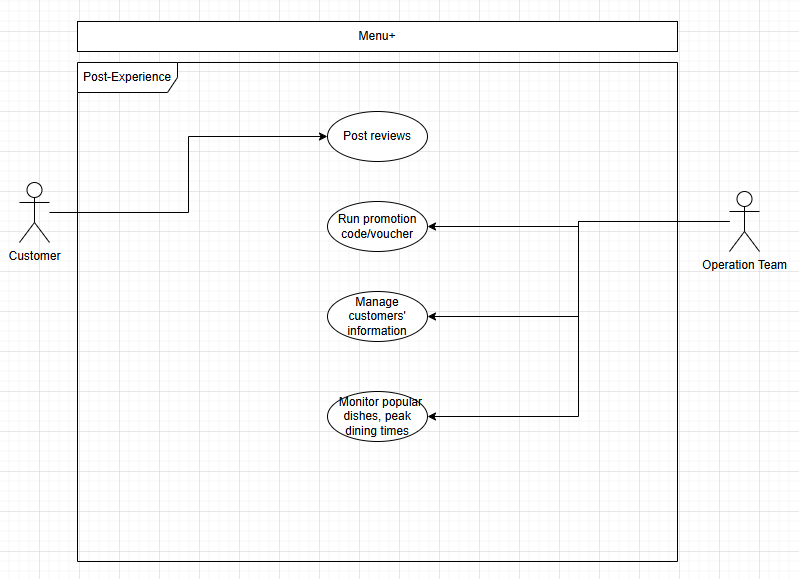
\includegraphics[width=\linewidth]{Images/ucd-postexp.png}
	\caption{Usecase Diagram giai đoạn Post-Experience}
        \end{figure}
        
        \begin{longtable}{|p{1cm}|p{5cm}|p{9cm}|}
        \hline
        \textbf{\#} & \textbf{Tên Use Case} & \textbf{Mô tả} \\ 
        \hline
        \endfirsthead
        \hline
        \textbf{\#} & \textbf{Tên Use Case} & \textbf{Mô tả} \\ 
        \endhead
        \hline
        % \multicolumn{3}{|r|}{\small\slshape Còn tiếp} \\ \hline
        \endfoot
        \hline
        \endlastfoot
        23 & Đăng đánh giá & Khách hàng có thể đăng đánh giá về trải nghiệm tại nhà hàng, bao gồm nhận xét về món ăn, dịch vụ, và không gian. \\ 
        \hline
        24 & Chạy chương trình khuyến mãi/mã giảm giá & Nhân viên vận hành (Operation Team) có thể thiết lập và chạy các chương trình khuyến mãi hoặc mã giảm giá để thu hút khách hàng. \\ 
        \hline
        25 & Quản lý thông tin khách hàng & Nhân viên vận hành có thể quản lý thông tin khách hàng (tên, số điện thoại, email, lịch sử đặt món, v.v.) để phục vụ tốt hơn. \\ 
        \hline
        26 & Theo dõi món ăn phổ biến, giờ cao điểm & Nhân viên vận hành có thể theo dõi dữ liệu về món ăn phổ biến và giờ cao điểm để tối ưu hóa hoạt động của nhà hàng. \\ 
        \hline
        \caption{Danh sách Use Case trong giai đoạn Post-Experience}\\
        \end{longtable}

        \begin{figure}[H]
	\centering
	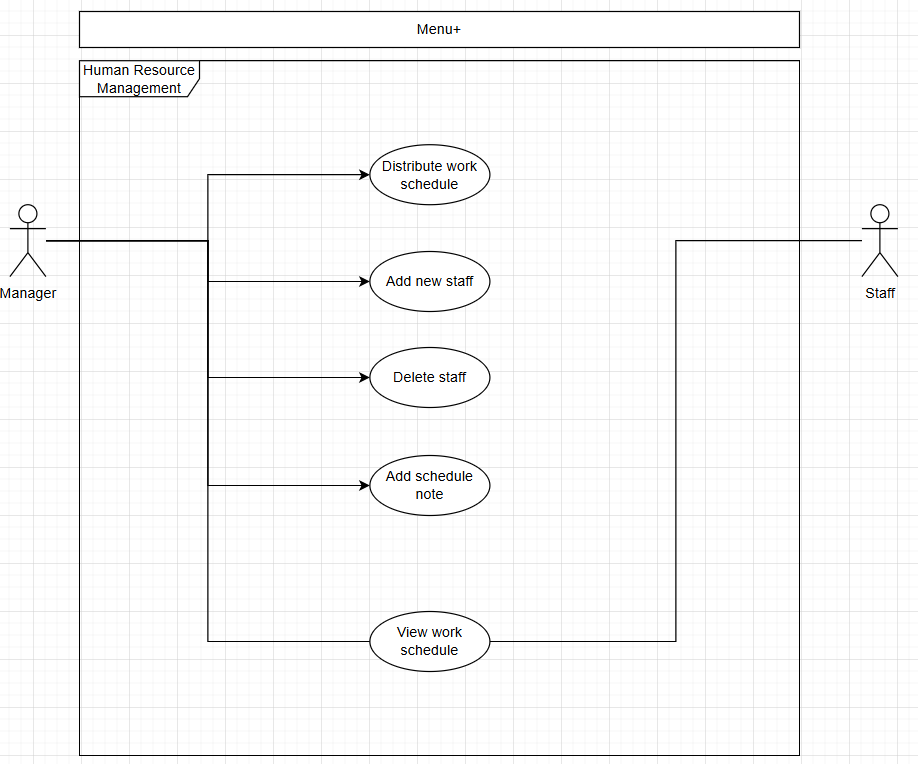
\includegraphics[width=\linewidth]{Images/ucd-hrm.png}
	\caption{Usecase Diagram phân hệ Human Resource Management}
        \end{figure}

        \begin{longtable}{|p{1cm}|p{5cm}|p{9cm}|}
        \hline
        \textbf{\#} & \textbf{Tên Use Case} & \textbf{Mô tả} \\ 
        \hline
        \endfirsthead
        \hline
        \textbf{\#} & \textbf{Tên Use Case} & \textbf{Mô tả} \\ 
        \endhead
        \hline
        % \multicolumn{3}{|r|}{\small\slshape Còn tiếp} \\ \hline
        \endfoot
        \hline
        \endlastfoot
        27 & Phân bổ lịch làm việc & Quản lý (Manager) có thể phân bổ lịch làm việc cho nhân viên, đảm bảo đủ nhân sự trong các ca làm việc. \\ 
        \hline
        28 & Thêm nhân viên mới & Quản lý có thể thêm thông tin nhân viên mới vào hệ thống, bao gồm tên, vị trí, và thông tin liên hệ. \\ 
        \hline
        29 & Xóa nhân viên & Quản lý có thể xóa thông tin nhân viên khỏi hệ thống nếu nhân viên không còn làm việc tại nhà hàng. \\ 
        \hline
        30 & Thêm ghi chú lịch trình & Quản lý có thể thêm ghi chú vào lịch làm việc của nhân viên, ví dụ: yêu cầu nghỉ phép, thay đổi ca làm, v.v. \\ 
        \hline
        31 & Xem lịch làm việc & Nhân viên (Staff) hoặc quản lý có thể xem lịch làm việc của mình để biết ca làm việc, thời gian và các ghi chú liên quan. \\ 
        \hline
        \caption{Danh sách Use Case trong phân hệ Human Resource Management}\\
        \end{longtable}

        \begin{figure}[H]
	\centering
	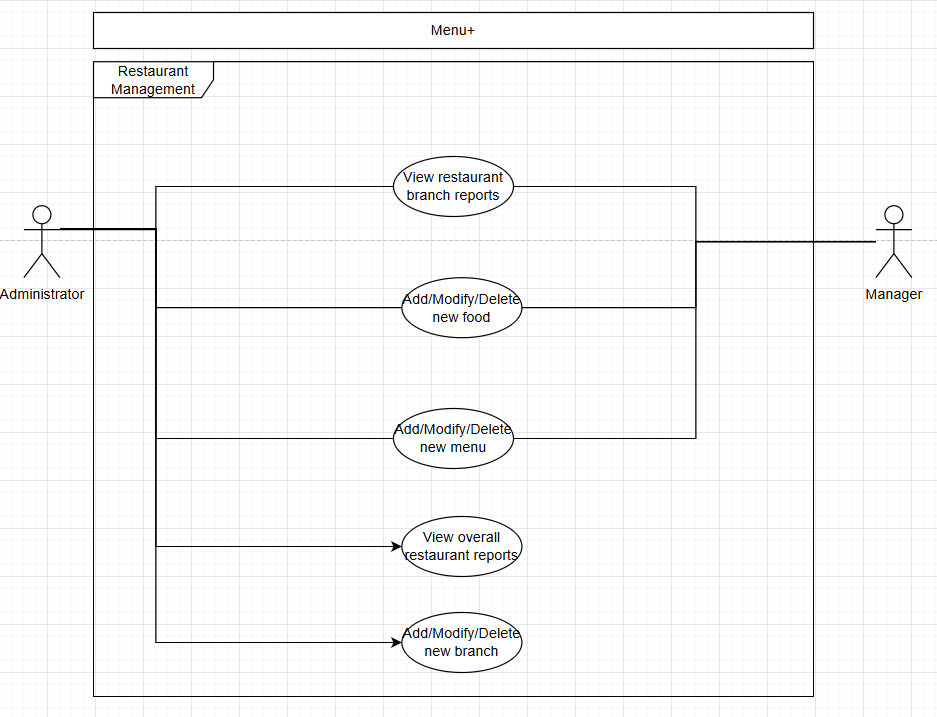
\includegraphics[width=\linewidth]{Images/ucd-rm.png}
	\caption{Usecase Diagram phân hệ Restaurant Management}
        \end{figure}
        
        \begin{longtable}{|p{1cm}|p{5cm}|p{9cm}|}
        \hline
        \textbf{\#} & \textbf{Tên Use Case} & \textbf{Mô tả} \\ 
        \hline
        \endfirsthead
        \hline
        \textbf{\#} & \textbf{Tên Use Case} & \textbf{Mô tả} \\ 
        \endhead
        \hline
        % \multicolumn{3}{|r|}{\small\slshape Còn tiếp} \\ \hline
        \endfoot
        \hline
        \endlastfoot
        32 & Xem báo cáo nhà hàng từng chi nhánh & Quản trị viên hoặc quản lý có thể xem báo cáo chi tiết về hoạt động của từng chi nhánh nhà hàng, bao gồm doanh thu, số lượng khách, v.v. \\ 
        \hline
        33 & Thêm/sửa/xóa món ăn mới & Quản trị viên hoặc quản lý có thể thêm, sửa hoặc xóa thông tin món ăn trong thực đơn, bao gồm tên món, giá, nguyên liệu, và mô tả. \\ 
        \hline
        34 & Thêm/sửa/xóa thực đơn mới & Quản trị viên hoặc quản lý có thể thêm, sửa hoặc xóa toàn bộ thực đơn mới, ví dụ: thực đơn theo mùa, thực đơn đặc biệt, v.v. \\ 
        \hline
        35 & Xem báo cáo tổng thể nhà hàng & Quản trị viên có thể xem báo cáo tổng thể về hoạt động của toàn bộ nhà hàng, bao gồm doanh thu, hiệu suất nhân viên, và các chỉ số khác. \\ 
        \hline
        36 & Thêm/sửa/xóa chi nhánh mới & Quản trị viên có thể thêm, sửa hoặc xóa thông tin về chi nhánh mới của nhà hàng, bao gồm địa chỉ, số điện thoại, và người quản lý chi nhánh. \\ 
        \hline
        \caption{Danh sách Use Case trong phân hệ Restaurant Management}\\
        \end{longtable}

    \subsubsection{Use Case chi tiết}
    \begin{itemize}
        \item \textbf{Xem thực đơn}
        
        \begin{longtable}{|p{3cm}|p{12cm}|}
        \hline
        \textbf{Tên Use Case} & \textbf{Xem thực đơn} \\ 
        \hline
        \endfirsthead
        \hline
        \textbf{Tên Use Case} & \textbf{Xem thực đơn} \\ 
        \endhead
        \hline
        \endfoot
        \hline
        \endlastfoot
        Actors & Guest (Khách hàng) \\ 
        \hline
        Description & Khách hàng xem danh sách các món ăn có sẵn trong thực đơn của nhà hàng, bao gồm thông tin về món ăn như giá cả, mô tả và hình ảnh. \\
        \hline
        Trigger & Khách hàng chọn chức năng "Xem thực đơn" trên ứng dụng hoặc giao diện của hệ thống Menu+. \\
        \hline
        Preconditions & - Hệ thống đã được khởi động và hoạt động bình thường.\newline- Thực đơn của nhà hàng đã được cập nhật và sẵn sàng hiển thị. \\
        \hline
        Postconditions & Khách hàng xem được danh sách món ăn và thông tin chi tiết, sẵn sàng để thực hiện các hành động tiếp theo như đặt món. \\
        \hline
        Normal Flow & 1. Khách hàng truy cập vào hệ thống Menu+.\newline2. Hệ thống hiển thị giao diện chính.\newline3. Khách hàng chọn chức năng "Xem thực đơn".\newline4. Hệ thống hiển thị danh sách các món ăn có sẵn, bao gồm tên món, giá cả, mô tả và hình ảnh (nếu có).\newline5. Khách hàng có thể cuộn hoặc tìm kiếm để xem các món ăn khác nhau.\newline6. Khách hàng chọn một món ăn để xem chi tiết (nếu muốn).\newline7. Hệ thống hiển thị thông tin chi tiết của món ăn (nguyên liệu, giá, tùy chọn tùy chỉnh, v.v.).\newline8. Khách hàng có thể quay lại danh sách thực đơn hoặc thoát khỏi chức năng xem thực đơn. \\
        \hline
        Alternative Flow & - Trường hợp 1: Ở bước 5, khách hàng sử dụng chức năng tìm kiếm để tìm món ăn theo tên hoặc danh mục (ví dụ: món chay, món chính). Hệ thống hiển thị kết quả tìm kiếm phù hợp, và khách hàng tiếp tục từ bước 6 nếu muốn xem chi tiết món ăn.\newline- Trường hợp 2: Ở bước 6, khách hàng không chọn xem chi tiết món ăn mà quay lại danh sách thực đơn ngay lập tức, tiếp tục cuộn để xem các món khác. \\
        \hline
        Exceptions & - Trường hợp 1: Ở bước 4, nếu thực đơn chưa được cập nhật hoặc không có món ăn nào, hệ thống hiển thị thông báo "Thực đơn hiện tại trống" và khách hàng quay lại giao diện chính.\newline- Trường hợp 2: Ở bước 4 hoặc 7, nếu hệ thống gặp lỗi kết nối (ví dụ: không tải được hình ảnh món ăn), hệ thống hiển thị thông báo lỗi "Không tải được dữ liệu, vui lòng thử lại" và cho phép khách hàng thử lại hoặc tiếp tục xem thông tin cơ bản (tên, giá, mô tả). \\
        \hline
        \caption{Use Case Schema cho Xem thực đơn}\\
        \end{longtable}
        
        \item \textbf{Đặt món ăn}\

        \begin{longtable}{|p{3cm}|p{12cm}|}
        \hline
        \textbf{Tên Use Case} & \textbf{Đặt món ăn} \\ 
        \hline
        \endfirsthead
        \hline
        \textbf{Tên Use Case} & \textbf{Đặt món ăn} \\ 
        \endhead
        \hline
        \endfoot
        \hline
        \endlastfoot
        Actors & Guest (Khách hàng), Waiter (Nhân viên phục vụ) \\ 
        \hline
        Description & Khách hàng đặt món ăn từ thực đơn của nhà hàng thông qua hệ thống Menu+, bao gồm các bước chọn món, thêm tùy chỉnh (nếu có), chọn hình thức đặt món (tại quán, mang đi, hoặc giao về), và xác nhận đơn hàng. Nhân viên phục vụ có thể hỗ trợ hoặc xác nhận đơn hàng. \\
        \hline
        Trigger & Khách hàng chọn chức năng "Đặt món ăn" sau khi xem thực đơn trên hệ thống Menu+. \\
        \hline
        Preconditions & - Hệ thống đã được khởi động và hoạt động bình thường.\newline- Khách hàng đã xem thực đơn và chọn được món ăn muốn đặt.\newline- Khách hàng đã đăng nhập (đối với hình thức giao về). \\
        \hline
        Postconditions & Đơn hàng của khách hàng được ghi nhận thành công trong hệ thống, bao gồm hình thức đặt món (tại quán, mang đi, hoặc giao về), và nhân viên phục vụ/đội bếp nhận được thông tin để chuẩn bị món ăn. \\
        \hline
        Normal Flow & 1. Khách hàng truy cập vào hệ thống Menu+.\newline2. Hệ thống hiển thị giao diện chính.\newline3. Khách hàng chọn chức năng "Đặt món ăn" (hoặc từ giao diện xem thực đơn, nhấn nút "Đặt món").\newline4. Hệ thống hiển thị danh sách món ăn để khách hàng lựa chọn.\newline5. Khách hàng chọn món ăn, số lượng, và thêm tùy chỉnh (nếu có, ví dụ: ít muối, không cay).\newline6. Hệ thống hiển thị giỏ hàng với các món đã chọn, bao gồm số lượng, tùy chỉnh, và tổng giá tạm tính.\newline7. Hệ thống yêu cầu khách hàng chọn hình thức đặt món: "Tại quán", "Mang đi", hoặc "Giao về".\newline8. Nếu chọn "Giao về", hệ thống yêu cầu khách hàng nhập thông tin giao hàng (địa chỉ, số điện thoại liên hệ).\newline9. Khách hàng xác nhận đơn hàng bằng cách nhấn "Gửi đơn hàng".\newline10. Hệ thống ghi nhận đơn hàng (bao gồm hình thức đặt món) và gửi thông tin đến nhân viên phục vụ/đội bếp.\newline11. Hệ thống hiển thị thông báo "Đơn hàng của bạn đã được ghi nhận" cho khách hàng, kèm theo thông tin về hình thức đặt món.\newline12. Nhân viên phục vụ nhận thông báo về đơn hàng và bắt đầu xử lý theo hình thức đã chọn. \\
        \hline
        Alternative Flow & - Trường hợp 1: Ở bước 5, khách hàng quyết định thêm món ăn khác trước khi xác nhận. Họ quay lại danh sách món ăn, chọn thêm món, và tiếp tục từ bước 6.\newline- Trường hợp 2: Ở bước 7, khách hàng thay đổi hình thức đặt món (ví dụ: từ "Tại quán" sang "Mang đi"). Hệ thống cập nhật lại giỏ hàng và tiếp tục từ bước 8 (nếu chọn "Giao về", yêu cầu nhập thông tin giao hàng).\newline- Trường hợp 3: Ở bước 9, khách hàng muốn chỉnh sửa đơn hàng (thay đổi số lượng, xóa món, hoặc thay đổi hình thức đặt món). Hệ thống cho phép chỉnh sửa trong giỏ hàng, sau đó khách hàng xác nhận lại và tiếp tục từ bước 10.\newline- Trường hợp 4: Ở bước 9, khách hàng hủy toàn bộ đơn hàng. Hệ thống xóa giỏ hàng và quay lại giao diện chính. \\
        \hline
        Exceptions & - Trường hợp 1: Ở bước 4, nếu danh sách món ăn không tải được do lỗi hệ thống, hệ thống hiển thị thông báo "Không tải được thực đơn, vui lòng thử lại" và cho phép khách hàng thử lại.\newline- Trường hợp 2: Ở bước 8, nếu khách hàng chọn "Giao về" nhưng không nhập đầy đủ thông tin giao hàng (ví dụ: thiếu địa chỉ), hệ thống hiển thị thông báo "Vui lòng nhập đầy đủ thông tin giao hàng" và yêu cầu nhập lại.\newline- Trường hợp 3: Ở bước 10, nếu hệ thống không gửi được đơn hàng đến nhân viên phục vụ/đội bếp do lỗi kết nối, hệ thống hiển thị thông báo "Lỗi gửi đơn hàng, vui lòng thử lại" và lưu tạm đơn hàng để khách hàng gửi lại. \\
        \hline
        \caption{Use Case Schema cho Đặt món ăn}\\
        \end{longtable}
        
        \item \textbf{Đặt bàn}

        \begin{longtable}{|p{3cm}|p{12cm}|}
        \hline
        \textbf{Tên Use Case} & \textbf{Đặt bàn} \\ 
        \hline
        \endfirsthead
        \hline
        \textbf{Tên Use Case} & \textbf{Đặt bàn} \\ 
        \endhead
        \hline
        \endfoot
        \hline
        \endlastfoot
        Actors & Guest (Khách hàng), Operation Team (Nhân viên vận hành) \\ 
        \hline
        Description & Khách hàng đặt bàn tại nhà hàng thông qua hệ thống Menu+, bao gồm các bước đăng nhập, chọn thời gian, số lượng người, và xác nhận đặt bàn. Nhân viên vận hành nhận thông tin để sắp xếp bàn. \\
        \hline
        Trigger & Khách hàng chọn chức năng "Đặt bàn" trên giao diện của hệ thống Menu+. \\
        \hline
        Preconditions & - Hệ thống đã được khởi động và hoạt động bình thường.\newline- Khách hàng đã có tài khoản và đăng nhập vào hệ thống.\newline- Nhà hàng có bàn trống trong khoảng thời gian khách hàng muốn đặt. \\
        \hline
        Postconditions & Đặt bàn được ghi nhận thành công trong hệ thống, khách hàng nhận được xác nhận, và nhân viên vận hành nhận thông tin để chuẩn bị bàn. \\
        \hline
        Normal Flow & 1. Khách hàng truy cập vào hệ thống Menu+.\newline2. Hệ thống hiển thị giao diện chính và yêu cầu khách hàng đăng nhập (nếu chưa đăng nhập).\newline3. Khách hàng nhập thông tin đăng nhập (tên người dùng/mật khẩu) và nhấn "Đăng nhập".\newline4. Hệ thống xác thực thông tin đăng nhập và cho phép truy cập.\newline5. Khách hàng chọn chức năng "Đặt bàn".\newline6. Hệ thống hiển thị giao diện đặt bàn, bao gồm các tùy chọn thời gian, số lượng người, và loại bàn (nếu có).\newline7. Khách hàng chọn thời gian đặt bàn, số lượng người, và loại bàn (nếu có sẵn).\newline8. Hệ thống kiểm tra tình trạng bàn trống và hiển thị xác nhận đặt bàn (bao gồm thời gian, số lượng người, và số bàn).\newline9. Khách hàng nhấn "Xác nhận đặt bàn".\newline10. Hệ thống ghi nhận đặt bàn và gửi thông tin đến nhân viên vận hành.\newline11. Hệ thống hiển thị thông báo "Đặt bàn thành công" cho khách hàng, kèm theo chi tiết đặt bàn (thời gian, số bàn, v.v.).\newline12. Nhân viên vận hành nhận thông báo về đặt bàn và chuẩn bị bàn cho khách hàng. \\
        \hline
        Alternative Flow & - Trường hợp 1: Ở bước 7, khách hàng thay đổi thời gian hoặc số lượng người trước khi xác nhận. Hệ thống cập nhật lại thông tin và kiểm tra tình trạng bàn trống, sau đó tiếp tục từ bước 8.\newline- Trường hợp 2: Ở bước 9, khách hàng hủy đặt bàn trước khi xác nhận. Hệ thống xóa thông tin đặt bàn và quay lại giao diện chính. \\
        \hline
        Exceptions & - Trường hợp 1: Ở bước 4, nếu thông tin đăng nhập không chính xác, hệ thống hiển thị thông báo "Tên người dùng hoặc mật khẩu không đúng, vui lòng thử lại" và yêu cầu khách hàng nhập lại.\newline- Trường hợp 2: Ở bước 8, nếu không có bàn trống trong thời gian khách hàng chọn, hệ thống hiển thị thông báo "Không có bàn trống vào thời gian này, vui lòng chọn thời gian khác" và quay lại bước 7.\newline- Trường hợp 3: Ở bước 10, nếu hệ thống không gửi được thông tin đặt bàn đến nhân viên vận hành do lỗi kết nối, hệ thống hiển thị thông báo "Lỗi ghi nhận đặt bàn, vui lòng thử lại" và lưu tạm thông tin để khách hàng gửi lại. \\
        \hline
        \caption{Use Case Schema cho Đặt bàn}\\
        \end{longtable}
        
        \item \textbf{Thay đổi trạng thái món ăn}

        \begin{longtable}{|p{3cm}|p{12cm}|}
        \hline
        \textbf{Tên Use Case} & \textbf{Thay đổi trạng thái món ăn} \\ 
        \hline
        \endfirsthead
        \hline
        \textbf{Tên Use Case} & \textbf{Thay đổi trạng thái món ăn} \\ 
        \endhead
        \hline
        \endfoot
        \hline
        \endlastfoot
        Actors & Waiter (Nhân viên phục vụ), Kitchen Team (Đội bếp) \\ 
        \hline
        Description & Nhân viên phục vụ hoặc đội bếp cập nhật trạng thái của món ăn trong đơn hàng (ví dụ: từ "Đang chuẩn bị" sang "Đã hoàn thành" hoặc "Đã phục vụ") để theo dõi tiến độ phục vụ. \\
        \hline
        Trigger & Nhân viên phục vụ hoặc đội bếp nhận được đơn hàng và cần cập nhật trạng thái món ăn trong quá trình xử lý. \\
        \hline
        Preconditions & - Hệ thống đã được khởi động và hoạt động bình thường.\newline- Đơn hàng đã được ghi nhận trong hệ thống.\newline- Nhân viên phục vụ hoặc đội bếp đã đăng nhập vào hệ thống. \\
        \hline
        Postconditions & Trạng thái món ăn được cập nhật thành công trong hệ thống, và các bên liên quan (nhân viên phục vụ, đội bếp) được thông báo về trạng thái mới. \\
        \hline
        Normal Flow & 1. Nhân viên phục vụ hoặc đội bếp đăng nhập vào hệ thống Menu+.\newline2. Hệ thống hiển thị danh sách đơn hàng đang xử lý.\newline3. Nhân viên chọn đơn hàng cần cập nhật trạng thái.\newline4. Hệ thống hiển thị chi tiết đơn hàng, bao gồm danh sách món ăn và trạng thái hiện tại (ví dụ: "Đang chuẩn bị").\newline5. Nhân viên chọn món ăn cần thay đổi trạng thái.\newline6. Nhân viên chọn trạng thái mới từ danh sách (ví dụ: "Đã hoàn thành", "Đã phục vụ").\newline7. Hệ thống cập nhật trạng thái món ăn và lưu vào cơ sở dữ liệu.\newline8. Hệ thống thông báo cho các bên liên quan (nhân viên phục vụ, đội bếp) về trạng thái mới. \\
        \hline
        Alternative Flow & - Trường hợp 1: Ở bước 6, nhân viên chọn nhầm trạng thái và muốn chỉnh sửa lại. Hệ thống cho phép chọn lại trạng thái trước khi xác nhận, sau đó tiếp tục từ bước 7.\newline- Trường hợp 2: Ở bước 3, nhân viên không tìm thấy đơn hàng cần cập nhật (do đã hoàn tất hoặc bị hủy). Hệ thống hiển thị thông báo "Đơn hàng không tồn tại" và quay lại bước 2. \\
        \hline
        Exceptions & - Trường hợp 1: Ở bước 7, nếu hệ thống gặp lỗi khi cập nhật trạng thái (ví dụ: lỗi kết nối), hệ thống hiển thị thông báo "Lỗi cập nhật trạng thái, vui lòng thử lại" và cho phép nhân viên thử lại.\newline- Trường hợp 2: Ở bước 8, nếu hệ thống không gửi được thông báo đến các bên liên quan do lỗi kết nối, hệ thống hiển thị thông báo "Lỗi gửi thông báo, trạng thái đã được cập nhật" và lưu trạng thái để kiểm tra sau. \\
        \hline
        \caption{Use Case Schema cho Thay đổi trạng thái món ăn}\\
        \end{longtable}
        
        \item \textbf{Xem danh sách bàn đã đặt}

        \begin{longtable}{|p{3cm}|p{12cm}|}
        \hline
        \textbf{Tên Use Case} & \textbf{Xem danh sách bàn đã đặt} \\ 
        \hline
        \endfirsthead
        \hline
        \textbf{Tên Use Case} & \textbf{Xem danh sách bàn đã đặt} \\ 
        \endhead
        \hline
        \endfoot
        \hline
        \endlastfoot
        Actors & Operation Team (Nhân viên vận hành) \\ 
        \hline
        Description & Nhân viên vận hành xem danh sách các bàn đã được đặt bởi khách hàng, bao gồm thông tin về thời gian đặt, số lượng người, và thông tin khách hàng (nếu có). \\
        \hline
        Trigger & Nhân viên vận hành chọn chức năng "Xem danh sách bàn đã đặt" trên giao diện hệ thống Menu+. \\
        \hline
        Preconditions & - Hệ thống đã được khởi động và hoạt động bình thường.\newline- Nhân viên vận hành đã đăng nhập vào hệ thống.\newline- Có ít nhất một đặt bàn đã được ghi nhận trong hệ thống. \\
        \hline
        Postconditions & Nhân viên vận hành xem được danh sách bàn đã đặt và thông tin chi tiết, sẵn sàng để sắp xếp hoặc xử lý các yêu cầu liên quan. \\
        \hline
        Normal Flow & 1. Nhân viên vận hành đăng nhập vào hệ thống Menu+.\newline2. Hệ thống hiển thị giao diện chính dành cho nhân viên.\newline3. Nhân viên chọn chức năng "Xem danh sách bàn đã đặt".\newline4. Hệ thống hiển thị danh sách các đặt bàn, bao gồm số bàn, thời gian đặt, số lượng người, và thông tin khách hàng (tên, số điện thoại).\newline5. Nhân viên chọn một đặt bàn để xem chi tiết (nếu cần).\newline6. Hệ thống hiển thị thông tin chi tiết của đặt bàn (ví dụ: yêu cầu đặc biệt, trạng thái bàn).\newline7. Nhân viên quay lại danh sách hoặc thoát khỏi chức năng. \\
        \hline
        Alternative Flow & - Trường hợp 1: Ở bước 4, nhân viên lọc danh sách đặt bàn theo thời gian (ví dụ: chỉ xem các đặt bàn trong buổi tối). Hệ thống hiển thị danh sách đã lọc, và nhân viên tiếp tục từ bước 5.\newline- Trường hợp 2: Ở bước 5, nhân viên không chọn xem chi tiết mà tiếp tục cuộn danh sách để kiểm tra các đặt bàn khác, sau đó quay lại bước 4 hoặc thoát. \\
        \hline
        Exceptions & - Trường hợp 1: Ở bước 4, nếu không có đặt bàn nào trong hệ thống, hệ thống hiển thị thông báo "Hiện tại không có đặt bàn nào" và quay lại giao diện chính.\newline- Trường hợp 2: Ở bước 4, nếu hệ thống gặp lỗi tải dữ liệu (ví dụ: lỗi kết nối), hệ thống hiển thị thông báo "Không tải được danh sách, vui lòng thử lại" và cho phép nhân viên thử lại. \\
        \hline
        \caption{Use Case Schema cho Xem danh sách bàn đã đặt}\\
        \end{longtable}

    \end{itemize}

    